

\section{Constructing a network from GTFS data}
\label{sec:route-segments}

In \cref{sec:literature}, I reported how arrival time prediction is greatly improved when data from multiple routes is combined to estimate traffic conditions \citep{Yu_2011}. However, many of these applications were specific to a certain set of routes, or used external information (such as automatic toll readers and taxis) to get \rt{} traffic information. We wanted to develop a \emph{simpler}, \emph{more generalised} approach using solely \GTFS{} data (stops and shapes) to construct a network of non-overlapping\footnote{Except of course reverse directions.} road segments. The network should consist of \emph{nodes} (which could be intersections or bus stops) connected by \emph{edges}, or road segments, which is similar to the structure used by \citet{Celan_2017,Vuurstaek_2018}.


The main goal of the network is to detect where any two routes overlap, even partially. There are several possible approaches to this, but the simplest is to look at common subsequences of bus stops. Of course, stops do not make optimal node locations because routes do not diverge \emph{physically} at stops---that would require locating \emph{intersections}. However, due to difficulties in finding intersections from either the \gls{gtfs} data or outside information, we opted to use bus stops for this work. \Cref{fig:gtfs_route_network} shows a simple route diagram with several overlapping routes. We see that each link between stops is common across routes, but routes that merge at intersections do not merge in the network until they reach a common stop.


\begin{knitrout}\small
\definecolor{shadecolor}{rgb}{1, 1, 1}\color{fgcolor}\begin{figure}

{\centering 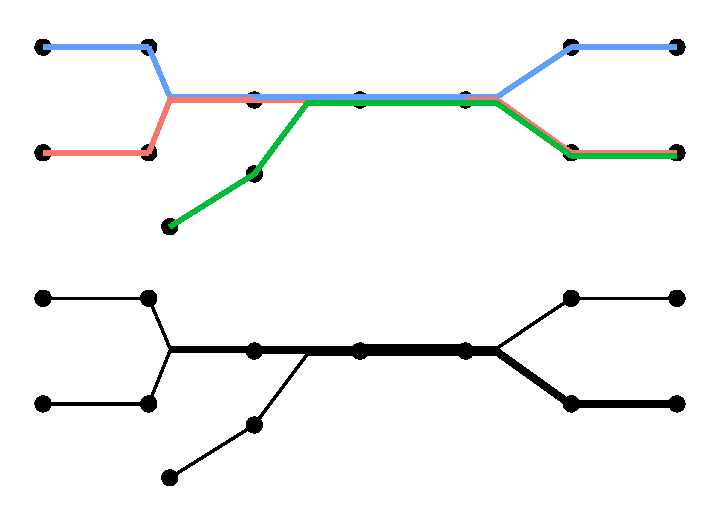
\includegraphics[width=0.6\textwidth]{figure/gtfs_route_network-1} 

}

\caption[A simplified transit network with road segments (edges) connecting stops (nodes)]{A simplified transit network with road segments (edges) connecting stops (nodes). Top: three routes with common subsequences of stops. Bottom: the widths of road segments represents the number of routes using them. There remains some segment overlap since routes merge at stops, not intersections.}\label{fig:gtfs_route_network}
\end{figure}


\end{knitrout}





One other issue with \AT{}'s \GTFS{} data is that all object IDs are \emph{versioned}. That is, instead of a route having an ID of \verb+02702+, the date and version number are appended to it: \verb+02702-20190806160740_v82.21+. This is the same for the IDs of trips, shapes, and stops, making it challenging to transfer existing segments based on stops from previous versions of the \gls{api} and requiring an additional step to remove the version information from the raw data.


The algorithm we implemented uses only bus stops but can extend to intersections, if available. Each stop along a route is assessed to see if any nodes already exist in that location to avoid the versioning issue mentioned above. If so, the route is assigned the existing node; otherwise, a new node is created and assigned instead. Road segments are defined by unique one-way connections between two stops: there can only be one segment going from node $A$ to node $B$ (the reverse is considered a different segment). The network is constructed within \pkg{transitr}:
\begin{knitrout}\small
\definecolor{shadecolor}{rgb}{1, 1, 1}\color{fgcolor}\begin{kframe}
\begin{alltt}
\hlkwd{library}\hlstd{(transitr)}
\hlstd{nw} \hlkwb{<-} \hlkwd{load_gtfs}\hlstd{(}\hlstr{"at_gtfs.sqlite"}\hlstd{)} \hlopt \hlkwd{construct}\hlstd{()}
\hlstd{transitr}\hlopt{:::}\hlkwd{load_road_segments}\hlstd{(nw)} \hlopt \hlkwd{head}\hlstd{()}
\end{alltt}
\begin{verbatim}
##   road_segment_id node_from node_to    length
## 1               1      5414     537  485.6548
## 2               2       537    3987  196.5567
## 3               3      3987    7265  567.0883
## 4               4      7265    1255 1049.0181
## 5               5      1255    4099  682.5452
## 6               6      4099    3436  535.0515
\end{verbatim}
\end{kframe}
\end{knitrout}
